
% Default to the notebook output style

    


% Inherit from the specified cell style.




    
\documentclass[11pt]{article}

    
    
    \usepackage[T1]{fontenc}
    % Nicer default font (+ math font) than Computer Modern for most use cases
    \usepackage{mathpazo}

    % Basic figure setup, for now with no caption control since it's done
    % automatically by Pandoc (which extracts ![](path) syntax from Markdown).
    \usepackage{graphicx}
    % We will generate all images so they have a width \maxwidth. This means
    % that they will get their normal width if they fit onto the page, but
    % are scaled down if they would overflow the margins.
    \makeatletter
    \def\maxwidth{\ifdim\Gin@nat@width>\linewidth\linewidth
    \else\Gin@nat@width\fi}
    \makeatother
    \let\Oldincludegraphics\includegraphics
    % Set max figure width to be 80% of text width, for now hardcoded.
    \renewcommand{\includegraphics}[1]{\Oldincludegraphics[width=.8\maxwidth]{#1}}
    % Ensure that by default, figures have no caption (until we provide a
    % proper Figure object with a Caption API and a way to capture that
    % in the conversion process - todo).
    \usepackage{caption}
    \DeclareCaptionLabelFormat{nolabel}{}
    \captionsetup{labelformat=nolabel}

    \usepackage{adjustbox} % Used to constrain images to a maximum size 
    \usepackage{xcolor} % Allow colors to be defined
    \usepackage{enumerate} % Needed for markdown enumerations to work
    \usepackage{geometry} % Used to adjust the document margins
    \usepackage{amsmath} % Equations
    \usepackage{amssymb} % Equations
    \usepackage{textcomp} % defines textquotesingle
    % Hack from http://tex.stackexchange.com/a/47451/13684:
    \AtBeginDocument{%
        \def\PYZsq{\textquotesingle}% Upright quotes in Pygmentized code
    }
    \usepackage{upquote} % Upright quotes for verbatim code
    \usepackage{eurosym} % defines \euro
    \usepackage[mathletters]{ucs} % Extended unicode (utf-8) support
    \usepackage[utf8x]{inputenc} % Allow utf-8 characters in the tex document
    \usepackage{fancyvrb} % verbatim replacement that allows latex
    \usepackage{grffile} % extends the file name processing of package graphics 
                         % to support a larger range 
    % The hyperref package gives us a pdf with properly built
    % internal navigation ('pdf bookmarks' for the table of contents,
    % internal cross-reference links, web links for URLs, etc.)
    \usepackage{hyperref}
    \usepackage{longtable} % longtable support required by pandoc >1.10
    \usepackage{booktabs}  % table support for pandoc > 1.12.2
    \usepackage[inline]{enumitem} % IRkernel/repr support (it uses the enumerate* environment)
    \usepackage[normalem]{ulem} % ulem is needed to support strikethroughs (\sout)
                                % normalem makes italics be italics, not underlines
    

    
    
    % Colors for the hyperref package
    \definecolor{urlcolor}{rgb}{0,.145,.698}
    \definecolor{linkcolor}{rgb}{.71,0.21,0.01}
    \definecolor{citecolor}{rgb}{.12,.54,.11}

    % ANSI colors
    \definecolor{ansi-black}{HTML}{3E424D}
    \definecolor{ansi-black-intense}{HTML}{282C36}
    \definecolor{ansi-red}{HTML}{E75C58}
    \definecolor{ansi-red-intense}{HTML}{B22B31}
    \definecolor{ansi-green}{HTML}{00A250}
    \definecolor{ansi-green-intense}{HTML}{007427}
    \definecolor{ansi-yellow}{HTML}{DDB62B}
    \definecolor{ansi-yellow-intense}{HTML}{B27D12}
    \definecolor{ansi-blue}{HTML}{208FFB}
    \definecolor{ansi-blue-intense}{HTML}{0065CA}
    \definecolor{ansi-magenta}{HTML}{D160C4}
    \definecolor{ansi-magenta-intense}{HTML}{A03196}
    \definecolor{ansi-cyan}{HTML}{60C6C8}
    \definecolor{ansi-cyan-intense}{HTML}{258F8F}
    \definecolor{ansi-white}{HTML}{C5C1B4}
    \definecolor{ansi-white-intense}{HTML}{A1A6B2}

    % commands and environments needed by pandoc snippets
    % extracted from the output of `pandoc -s`
    \providecommand{\tightlist}{%
      \setlength{\itemsep}{0pt}\setlength{\parskip}{0pt}}
    \DefineVerbatimEnvironment{Highlighting}{Verbatim}{commandchars=\\\{\}}
    % Add ',fontsize=\small' for more characters per line
    \newenvironment{Shaded}{}{}
    \newcommand{\KeywordTok}[1]{\textcolor[rgb]{0.00,0.44,0.13}{\textbf{{#1}}}}
    \newcommand{\DataTypeTok}[1]{\textcolor[rgb]{0.56,0.13,0.00}{{#1}}}
    \newcommand{\DecValTok}[1]{\textcolor[rgb]{0.25,0.63,0.44}{{#1}}}
    \newcommand{\BaseNTok}[1]{\textcolor[rgb]{0.25,0.63,0.44}{{#1}}}
    \newcommand{\FloatTok}[1]{\textcolor[rgb]{0.25,0.63,0.44}{{#1}}}
    \newcommand{\CharTok}[1]{\textcolor[rgb]{0.25,0.44,0.63}{{#1}}}
    \newcommand{\StringTok}[1]{\textcolor[rgb]{0.25,0.44,0.63}{{#1}}}
    \newcommand{\CommentTok}[1]{\textcolor[rgb]{0.38,0.63,0.69}{\textit{{#1}}}}
    \newcommand{\OtherTok}[1]{\textcolor[rgb]{0.00,0.44,0.13}{{#1}}}
    \newcommand{\AlertTok}[1]{\textcolor[rgb]{1.00,0.00,0.00}{\textbf{{#1}}}}
    \newcommand{\FunctionTok}[1]{\textcolor[rgb]{0.02,0.16,0.49}{{#1}}}
    \newcommand{\RegionMarkerTok}[1]{{#1}}
    \newcommand{\ErrorTok}[1]{\textcolor[rgb]{1.00,0.00,0.00}{\textbf{{#1}}}}
    \newcommand{\NormalTok}[1]{{#1}}
    
    % Additional commands for more recent versions of Pandoc
    \newcommand{\ConstantTok}[1]{\textcolor[rgb]{0.53,0.00,0.00}{{#1}}}
    \newcommand{\SpecialCharTok}[1]{\textcolor[rgb]{0.25,0.44,0.63}{{#1}}}
    \newcommand{\VerbatimStringTok}[1]{\textcolor[rgb]{0.25,0.44,0.63}{{#1}}}
    \newcommand{\SpecialStringTok}[1]{\textcolor[rgb]{0.73,0.40,0.53}{{#1}}}
    \newcommand{\ImportTok}[1]{{#1}}
    \newcommand{\DocumentationTok}[1]{\textcolor[rgb]{0.73,0.13,0.13}{\textit{{#1}}}}
    \newcommand{\AnnotationTok}[1]{\textcolor[rgb]{0.38,0.63,0.69}{\textbf{\textit{{#1}}}}}
    \newcommand{\CommentVarTok}[1]{\textcolor[rgb]{0.38,0.63,0.69}{\textbf{\textit{{#1}}}}}
    \newcommand{\VariableTok}[1]{\textcolor[rgb]{0.10,0.09,0.49}{{#1}}}
    \newcommand{\ControlFlowTok}[1]{\textcolor[rgb]{0.00,0.44,0.13}{\textbf{{#1}}}}
    \newcommand{\OperatorTok}[1]{\textcolor[rgb]{0.40,0.40,0.40}{{#1}}}
    \newcommand{\BuiltInTok}[1]{{#1}}
    \newcommand{\ExtensionTok}[1]{{#1}}
    \newcommand{\PreprocessorTok}[1]{\textcolor[rgb]{0.74,0.48,0.00}{{#1}}}
    \newcommand{\AttributeTok}[1]{\textcolor[rgb]{0.49,0.56,0.16}{{#1}}}
    \newcommand{\InformationTok}[1]{\textcolor[rgb]{0.38,0.63,0.69}{\textbf{\textit{{#1}}}}}
    \newcommand{\WarningTok}[1]{\textcolor[rgb]{0.38,0.63,0.69}{\textbf{\textit{{#1}}}}}
    
    
    % Define a nice break command that doesn't care if a line doesn't already
    % exist.
    \def\br{\hspace*{\fill} \\* }
    % Math Jax compatability definitions
    \def\gt{>}
    \def\lt{<}
    % Document parameters
    \title{Ejercicio 1}
    
    
    

    % Pygments definitions
    
\makeatletter
\def\PY@reset{\let\PY@it=\relax \let\PY@bf=\relax%
    \let\PY@ul=\relax \let\PY@tc=\relax%
    \let\PY@bc=\relax \let\PY@ff=\relax}
\def\PY@tok#1{\csname PY@tok@#1\endcsname}
\def\PY@toks#1+{\ifx\relax#1\empty\else%
    \PY@tok{#1}\expandafter\PY@toks\fi}
\def\PY@do#1{\PY@bc{\PY@tc{\PY@ul{%
    \PY@it{\PY@bf{\PY@ff{#1}}}}}}}
\def\PY#1#2{\PY@reset\PY@toks#1+\relax+\PY@do{#2}}

\expandafter\def\csname PY@tok@w\endcsname{\def\PY@tc##1{\textcolor[rgb]{0.73,0.73,0.73}{##1}}}
\expandafter\def\csname PY@tok@c\endcsname{\let\PY@it=\textit\def\PY@tc##1{\textcolor[rgb]{0.25,0.50,0.50}{##1}}}
\expandafter\def\csname PY@tok@cp\endcsname{\def\PY@tc##1{\textcolor[rgb]{0.74,0.48,0.00}{##1}}}
\expandafter\def\csname PY@tok@k\endcsname{\let\PY@bf=\textbf\def\PY@tc##1{\textcolor[rgb]{0.00,0.50,0.00}{##1}}}
\expandafter\def\csname PY@tok@kp\endcsname{\def\PY@tc##1{\textcolor[rgb]{0.00,0.50,0.00}{##1}}}
\expandafter\def\csname PY@tok@kt\endcsname{\def\PY@tc##1{\textcolor[rgb]{0.69,0.00,0.25}{##1}}}
\expandafter\def\csname PY@tok@o\endcsname{\def\PY@tc##1{\textcolor[rgb]{0.40,0.40,0.40}{##1}}}
\expandafter\def\csname PY@tok@ow\endcsname{\let\PY@bf=\textbf\def\PY@tc##1{\textcolor[rgb]{0.67,0.13,1.00}{##1}}}
\expandafter\def\csname PY@tok@nb\endcsname{\def\PY@tc##1{\textcolor[rgb]{0.00,0.50,0.00}{##1}}}
\expandafter\def\csname PY@tok@nf\endcsname{\def\PY@tc##1{\textcolor[rgb]{0.00,0.00,1.00}{##1}}}
\expandafter\def\csname PY@tok@nc\endcsname{\let\PY@bf=\textbf\def\PY@tc##1{\textcolor[rgb]{0.00,0.00,1.00}{##1}}}
\expandafter\def\csname PY@tok@nn\endcsname{\let\PY@bf=\textbf\def\PY@tc##1{\textcolor[rgb]{0.00,0.00,1.00}{##1}}}
\expandafter\def\csname PY@tok@ne\endcsname{\let\PY@bf=\textbf\def\PY@tc##1{\textcolor[rgb]{0.82,0.25,0.23}{##1}}}
\expandafter\def\csname PY@tok@nv\endcsname{\def\PY@tc##1{\textcolor[rgb]{0.10,0.09,0.49}{##1}}}
\expandafter\def\csname PY@tok@no\endcsname{\def\PY@tc##1{\textcolor[rgb]{0.53,0.00,0.00}{##1}}}
\expandafter\def\csname PY@tok@nl\endcsname{\def\PY@tc##1{\textcolor[rgb]{0.63,0.63,0.00}{##1}}}
\expandafter\def\csname PY@tok@ni\endcsname{\let\PY@bf=\textbf\def\PY@tc##1{\textcolor[rgb]{0.60,0.60,0.60}{##1}}}
\expandafter\def\csname PY@tok@na\endcsname{\def\PY@tc##1{\textcolor[rgb]{0.49,0.56,0.16}{##1}}}
\expandafter\def\csname PY@tok@nt\endcsname{\let\PY@bf=\textbf\def\PY@tc##1{\textcolor[rgb]{0.00,0.50,0.00}{##1}}}
\expandafter\def\csname PY@tok@nd\endcsname{\def\PY@tc##1{\textcolor[rgb]{0.67,0.13,1.00}{##1}}}
\expandafter\def\csname PY@tok@s\endcsname{\def\PY@tc##1{\textcolor[rgb]{0.73,0.13,0.13}{##1}}}
\expandafter\def\csname PY@tok@sd\endcsname{\let\PY@it=\textit\def\PY@tc##1{\textcolor[rgb]{0.73,0.13,0.13}{##1}}}
\expandafter\def\csname PY@tok@si\endcsname{\let\PY@bf=\textbf\def\PY@tc##1{\textcolor[rgb]{0.73,0.40,0.53}{##1}}}
\expandafter\def\csname PY@tok@se\endcsname{\let\PY@bf=\textbf\def\PY@tc##1{\textcolor[rgb]{0.73,0.40,0.13}{##1}}}
\expandafter\def\csname PY@tok@sr\endcsname{\def\PY@tc##1{\textcolor[rgb]{0.73,0.40,0.53}{##1}}}
\expandafter\def\csname PY@tok@ss\endcsname{\def\PY@tc##1{\textcolor[rgb]{0.10,0.09,0.49}{##1}}}
\expandafter\def\csname PY@tok@sx\endcsname{\def\PY@tc##1{\textcolor[rgb]{0.00,0.50,0.00}{##1}}}
\expandafter\def\csname PY@tok@m\endcsname{\def\PY@tc##1{\textcolor[rgb]{0.40,0.40,0.40}{##1}}}
\expandafter\def\csname PY@tok@gh\endcsname{\let\PY@bf=\textbf\def\PY@tc##1{\textcolor[rgb]{0.00,0.00,0.50}{##1}}}
\expandafter\def\csname PY@tok@gu\endcsname{\let\PY@bf=\textbf\def\PY@tc##1{\textcolor[rgb]{0.50,0.00,0.50}{##1}}}
\expandafter\def\csname PY@tok@gd\endcsname{\def\PY@tc##1{\textcolor[rgb]{0.63,0.00,0.00}{##1}}}
\expandafter\def\csname PY@tok@gi\endcsname{\def\PY@tc##1{\textcolor[rgb]{0.00,0.63,0.00}{##1}}}
\expandafter\def\csname PY@tok@gr\endcsname{\def\PY@tc##1{\textcolor[rgb]{1.00,0.00,0.00}{##1}}}
\expandafter\def\csname PY@tok@ge\endcsname{\let\PY@it=\textit}
\expandafter\def\csname PY@tok@gs\endcsname{\let\PY@bf=\textbf}
\expandafter\def\csname PY@tok@gp\endcsname{\let\PY@bf=\textbf\def\PY@tc##1{\textcolor[rgb]{0.00,0.00,0.50}{##1}}}
\expandafter\def\csname PY@tok@go\endcsname{\def\PY@tc##1{\textcolor[rgb]{0.53,0.53,0.53}{##1}}}
\expandafter\def\csname PY@tok@gt\endcsname{\def\PY@tc##1{\textcolor[rgb]{0.00,0.27,0.87}{##1}}}
\expandafter\def\csname PY@tok@err\endcsname{\def\PY@bc##1{\setlength{\fboxsep}{0pt}\fcolorbox[rgb]{1.00,0.00,0.00}{1,1,1}{\strut ##1}}}
\expandafter\def\csname PY@tok@kc\endcsname{\let\PY@bf=\textbf\def\PY@tc##1{\textcolor[rgb]{0.00,0.50,0.00}{##1}}}
\expandafter\def\csname PY@tok@kd\endcsname{\let\PY@bf=\textbf\def\PY@tc##1{\textcolor[rgb]{0.00,0.50,0.00}{##1}}}
\expandafter\def\csname PY@tok@kn\endcsname{\let\PY@bf=\textbf\def\PY@tc##1{\textcolor[rgb]{0.00,0.50,0.00}{##1}}}
\expandafter\def\csname PY@tok@kr\endcsname{\let\PY@bf=\textbf\def\PY@tc##1{\textcolor[rgb]{0.00,0.50,0.00}{##1}}}
\expandafter\def\csname PY@tok@bp\endcsname{\def\PY@tc##1{\textcolor[rgb]{0.00,0.50,0.00}{##1}}}
\expandafter\def\csname PY@tok@fm\endcsname{\def\PY@tc##1{\textcolor[rgb]{0.00,0.00,1.00}{##1}}}
\expandafter\def\csname PY@tok@vc\endcsname{\def\PY@tc##1{\textcolor[rgb]{0.10,0.09,0.49}{##1}}}
\expandafter\def\csname PY@tok@vg\endcsname{\def\PY@tc##1{\textcolor[rgb]{0.10,0.09,0.49}{##1}}}
\expandafter\def\csname PY@tok@vi\endcsname{\def\PY@tc##1{\textcolor[rgb]{0.10,0.09,0.49}{##1}}}
\expandafter\def\csname PY@tok@vm\endcsname{\def\PY@tc##1{\textcolor[rgb]{0.10,0.09,0.49}{##1}}}
\expandafter\def\csname PY@tok@sa\endcsname{\def\PY@tc##1{\textcolor[rgb]{0.73,0.13,0.13}{##1}}}
\expandafter\def\csname PY@tok@sb\endcsname{\def\PY@tc##1{\textcolor[rgb]{0.73,0.13,0.13}{##1}}}
\expandafter\def\csname PY@tok@sc\endcsname{\def\PY@tc##1{\textcolor[rgb]{0.73,0.13,0.13}{##1}}}
\expandafter\def\csname PY@tok@dl\endcsname{\def\PY@tc##1{\textcolor[rgb]{0.73,0.13,0.13}{##1}}}
\expandafter\def\csname PY@tok@s2\endcsname{\def\PY@tc##1{\textcolor[rgb]{0.73,0.13,0.13}{##1}}}
\expandafter\def\csname PY@tok@sh\endcsname{\def\PY@tc##1{\textcolor[rgb]{0.73,0.13,0.13}{##1}}}
\expandafter\def\csname PY@tok@s1\endcsname{\def\PY@tc##1{\textcolor[rgb]{0.73,0.13,0.13}{##1}}}
\expandafter\def\csname PY@tok@mb\endcsname{\def\PY@tc##1{\textcolor[rgb]{0.40,0.40,0.40}{##1}}}
\expandafter\def\csname PY@tok@mf\endcsname{\def\PY@tc##1{\textcolor[rgb]{0.40,0.40,0.40}{##1}}}
\expandafter\def\csname PY@tok@mh\endcsname{\def\PY@tc##1{\textcolor[rgb]{0.40,0.40,0.40}{##1}}}
\expandafter\def\csname PY@tok@mi\endcsname{\def\PY@tc##1{\textcolor[rgb]{0.40,0.40,0.40}{##1}}}
\expandafter\def\csname PY@tok@il\endcsname{\def\PY@tc##1{\textcolor[rgb]{0.40,0.40,0.40}{##1}}}
\expandafter\def\csname PY@tok@mo\endcsname{\def\PY@tc##1{\textcolor[rgb]{0.40,0.40,0.40}{##1}}}
\expandafter\def\csname PY@tok@ch\endcsname{\let\PY@it=\textit\def\PY@tc##1{\textcolor[rgb]{0.25,0.50,0.50}{##1}}}
\expandafter\def\csname PY@tok@cm\endcsname{\let\PY@it=\textit\def\PY@tc##1{\textcolor[rgb]{0.25,0.50,0.50}{##1}}}
\expandafter\def\csname PY@tok@cpf\endcsname{\let\PY@it=\textit\def\PY@tc##1{\textcolor[rgb]{0.25,0.50,0.50}{##1}}}
\expandafter\def\csname PY@tok@c1\endcsname{\let\PY@it=\textit\def\PY@tc##1{\textcolor[rgb]{0.25,0.50,0.50}{##1}}}
\expandafter\def\csname PY@tok@cs\endcsname{\let\PY@it=\textit\def\PY@tc##1{\textcolor[rgb]{0.25,0.50,0.50}{##1}}}

\def\PYZbs{\char`\\}
\def\PYZus{\char`\_}
\def\PYZob{\char`\{}
\def\PYZcb{\char`\}}
\def\PYZca{\char`\^}
\def\PYZam{\char`\&}
\def\PYZlt{\char`\<}
\def\PYZgt{\char`\>}
\def\PYZsh{\char`\#}
\def\PYZpc{\char`\%}
\def\PYZdl{\char`\$}
\def\PYZhy{\char`\-}
\def\PYZsq{\char`\'}
\def\PYZdq{\char`\"}
\def\PYZti{\char`\~}
% for compatibility with earlier versions
\def\PYZat{@}
\def\PYZlb{[}
\def\PYZrb{]}
\makeatother


    % Exact colors from NB
    \definecolor{incolor}{rgb}{0.0, 0.0, 0.5}
    \definecolor{outcolor}{rgb}{0.545, 0.0, 0.0}



    
    % Prevent overflowing lines due to hard-to-break entities
    \sloppy 
    % Setup hyperref package
    \hypersetup{
      breaklinks=true,  % so long urls are correctly broken across lines
      colorlinks=true,
      urlcolor=urlcolor,
      linkcolor=linkcolor,
      citecolor=citecolor,
      }
    % Slightly bigger margins than the latex defaults
    
    \geometry{verbose,tmargin=1in,bmargin=1in,lmargin=1in,rmargin=1in}
    
    

    \begin{document}
    \title{Practica 2}
    \author{González Borja, Miguel \\ Illescas Arizti, Rodrigo \\ Meyer Mañón, Juan Carlos\\ Rodríguez Orozco, Alejandro}
    \date{28 / Abril / 2018}
    \graphicspath{{../Graficas/}}
    \maketitle
    
    \section*{Introducci\'on}
A continuación los ejercicios de la práctica. Todos fueron realizados en Python 3.6 utilizando los paquetes \textit{numpy} y \textit{scipy.optimize}. También se incluye un cuaderno de IPython para cada ejercicio dentro de la carpeta Ejercicios, junto con los scripts \textit{.py} para obtener los resultados. Cada uno de estos utiliza los siguientes imports:

    
    \begin{Verbatim}[commandchars=\\\{\}]
{\color{incolor}In [{\color{incolor}1}]:} \PY{k+kn}{import} \PY{n+nn}{sys}
        \PY{n}{sys}\PY{o}{.}\PY{n}{path}\PY{o}{.}\PY{n}{append}\PY{p}{(}\PY{l+s+s1}{\PYZsq{}}\PY{l+s+s1}{../}\PY{l+s+s1}{\PYZsq{}}\PY{p}{)}
        \PY{k+kn}{import} \PY{n+nn}{latexStrings} \PY{k}{as} \PY{n+nn}{ls}
        \PY{k+kn}{import} \PY{n+nn}{numpy} \PY{k}{as} \PY{n+nn}{np}
        \PY{k+kn}{import} \PY{n+nn}{matplotlib}\PY{n+nn}{.}\PY{n+nn}{pyplot} \PY{k}{as} \PY{n+nn}{plt}
        \PY{k+kn}{from} \PY{n+nn}{math} \PY{k}{import} \PY{o}{*}
        \PY{k+kn}{from} \PY{n+nn}{IPython}\PY{n+nn}{.}\PY{n+nn}{display} \PY{k}{import} \PY{n}{Latex}
        \PY{k+kn}{import} \PY{n+nn}{odesolver}
\end{Verbatim}
Se puede encontrar un repositorio del proyecto \href{https://github.com/ekiMGlz/ODEMethods}{aqui}.

    \section*{Ejercicio 1}\label{ejercicio-1}

    Tenemos el PVI:

\begin{equation} \label{eq:1}
y'= y + 2e^{-t} \qquad y(0) = 1 
\end{equation}

Dado que el lado derecho de la EDO, \(y + 2e^{-t}\) es de clase \(C^1\)
para todo \((t,y)\in \mathbb{R}\times\mathbb{R}\), y por lo tanto
Lipschitz Continua en dicha region, sabemos que existe una solucion
unica a este problema, que en general es dada por:

\begin{equation} \label{eq:2}
y(t) = (y_0e^{-t_0} + e^{-2t_0}-e^{-2t})e^t
\end{equation}

Ahora apliquemos el metodo de Euler Explicito con paso \(h=0.1\):

    \begin{Verbatim}[commandchars=\\\{\}]
{\color{incolor}In [{\color{incolor}1}]:} \PY{n}{f} \PY{o}{=} \PY{k}{lambda} \PY{n}{t}\PY{p}{,} \PY{n}{y} \PY{p}{:} \PY{n}{y}\PY{o}{+}\PY{l+m+mi}{2}\PY{o}{*}\PY{n}{np}\PY{o}{.}\PY{n}{exp}\PY{p}{(}\PY{o}{\PYZhy{}}\PY{n}{t}\PY{p}{)}
        \PY{n}{exact} \PY{o}{=} \PY{k}{lambda} \PY{n}{t}\PY{p}{,} \PY{n}{t0}\PY{p}{,} \PY{n}{y0} \PY{p}{:} \PY{n}{np}\PY{o}{.}\PY{n}{exp}\PY{p}{(}\PY{n}{t}\PY{p}{)}\PY{o}{*}\PY{p}{(}\PY{n}{y0}\PY{o}{*}\PY{n}{np}\PY{o}{.}\PY{n}{exp}\PY{p}{(}\PY{o}{\PYZhy{}}\PY{n}{t0}\PY{p}{)}\PY{o}{+}\PY{n}{np}\PY{o}{.}\PY{n}{exp}\PY{p}{(}\PY{o}{\PYZhy{}}\PY{l+m+mi}{2}\PY{o}{*}\PY{n}{t0}\PY{p}{)}\PY{o}{\PYZhy{}}\PY{n}{np}\PY{o}{.}\PY{n}{exp}\PY{p}{(}\PY{o}{\PYZhy{}}\PY{l+m+mi}{2}\PY{o}{*}\PY{n}{t}\PY{p}{)}\PY{p}{)}
        \PY{n}{I} \PY{o}{=} \PY{p}{(}\PY{l+m+mi}{0}\PY{p}{,} \PY{l+m+mi}{1}\PY{p}{)}
        \PY{n}{y0} \PY{o}{=} \PY{l+m+mi}{1}
        \PY{n}{y1} \PY{o}{=} \PY{n}{exact}\PY{p}{(}\PY{l+m+mi}{1}\PY{p}{,}\PY{l+m+mi}{0}\PY{p}{,}\PY{l+m+mi}{1}\PY{p}{)}
        \PY{n}{T}\PY{p}{,} \PY{n}{W} \PY{o}{=} \PY{n}{odesolver}\PY{o}{.}\PY{n}{solve}\PY{p}{(}\PY{n}{f}\PY{p}{,}\PY{n}{y0}\PY{p}{,}\PY{n}{I}\PY{p}{,}\PY{l+m+mi}{10}\PY{p}{,}\PY{n}{method}\PY{o}{=}\PY{l+s+s2}{\PYZdq{}}\PY{l+s+s2}{Explicit Euler}\PY{l+s+s2}{\PYZdq{}}\PY{p}{)}
        \PY{n}{globalError} \PY{o}{=} \PY{n+nb}{abs}\PY{p}{(}\PY{n}{W}\PY{p}{[}\PY{l+m+mi}{0}\PY{p}{,}\PY{l+m+mi}{10}\PY{p}{]}\PY{o}{\PYZhy{}}\PY{n}{y1}\PY{p}{)}
        \PY{n}{localErrors} \PY{o}{=} \PY{p}{[}\PY{n+nb}{abs}\PY{p}{(}\PY{n}{W}\PY{p}{[}\PY{l+m+mi}{0}\PY{p}{,}\PY{n}{i}\PY{o}{+}\PY{l+m+mi}{1}\PY{p}{]} \PY{o}{\PYZhy{}} \PY{n}{exact}\PY{p}{(}\PY{n}{T}\PY{p}{[}\PY{n}{i}\PY{o}{+}\PY{l+m+mi}{1}\PY{p}{]}\PY{p}{,} \PY{n}{T}\PY{p}{[}\PY{n}{i}\PY{p}{]}\PY{p}{,} \PY{n}{W}\PY{p}{[}\PY{l+m+mi}{0}\PY{p}{,}\PY{n}{i}\PY{p}{]}\PY{p}{)}\PY{p}{)} \PY{k}{for} \PY{n}{i} \PY{o+ow}{in} \PY{n+nb}{range}\PY{p}{(}\PY{l+m+mi}{10}\PY{p}{)}\PY{p}{]}
        \PY{n}{maxLocalError} \PY{o}{=} \PY{n+nb}{max}\PY{p}{(}\PY{n}{localErrors}\PY{p}{)}
\end{Verbatim}
\begin{align*}
 w =&\{ 
1, 1.3, 1.6109675, 1.9358104, 2.2775551, 2.6393746,\\ 
&3.0246182, 3.4368423, 3.8798436, 4.3576938, 4.8747771\}\\
 \text{Error Global: } &0.1939071469339151\\
\text{ Maximo Error Local: } &0.022668868433444622
\end{align*}
    

    Graficamente, observemos como se comporta la solucion exacta contra la
aproximada:
    \begin{center}
    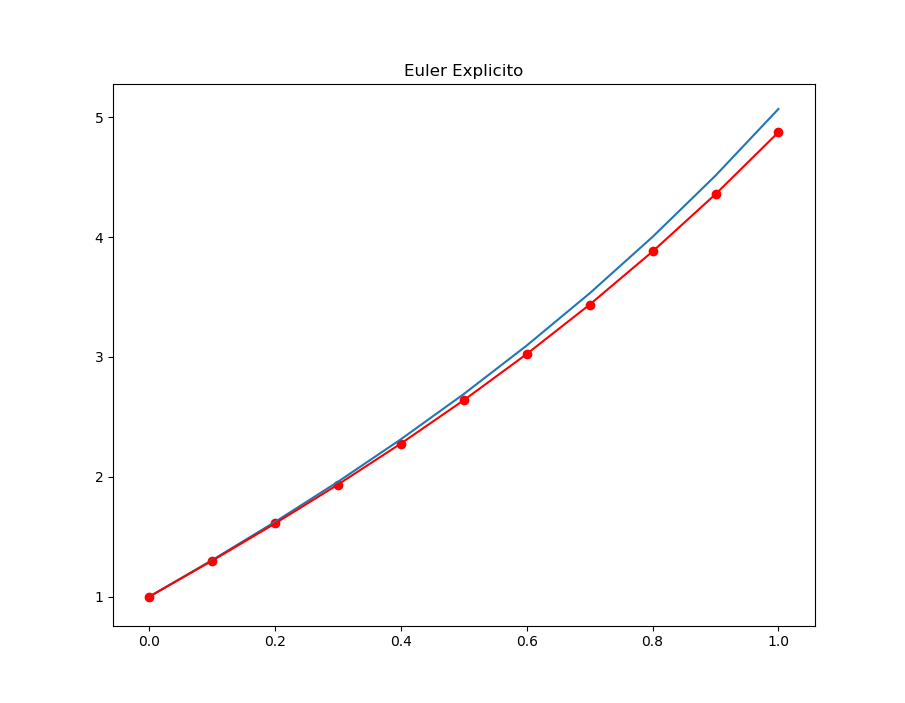
\includegraphics{fig 1.1.png}
    \end{center}
    { \hspace*{\fill} \\}
    
    Vemos que la solucion aproximada, auque sigue la direccion general,
siempre va por debajo de la solucion verdadera. Esto se debe a que
nuestra solucion general (\ref{eq:2}) es convexa en el intervalo donde
estamos buscando la solucion, y por lo tanto el metodo subestima la
pendiente en sus aproximaciones.

Ahora apliquemos el metodo de Euler Explicito con pasos
\(h = 0.1 \times 2^{-k}\) para \(k \in \{0,1,\dots, 5\}\) en el
intervalo \([0,1]\):

    \begin{Verbatim}[commandchars=\\\{\}]
{\color{incolor}In [{\color{incolor}2}]:} \PY{n}{res} \PY{o}{=} \PY{p}{[}\PY{p}{]}
        \PY{n}{globalErrors}\PY{o}{=}\PY{p}{[}\PY{p}{]}
        \PY{k}{for} \PY{n}{k} \PY{o+ow}{in} \PY{n+nb}{range}\PY{p}{(}\PY{l+m+mi}{6}\PY{p}{)}\PY{p}{:}
            \PY{n}{h} \PY{o}{=} \PY{l+m+mf}{0.1}\PY{o}{*}\PY{p}{(}\PY{l+m+mi}{2}\PY{o}{*}\PY{o}{*}\PY{o}{\PYZhy{}}\PY{n}{k}\PY{p}{)}
            \PY{n}{m} \PY{o}{=} \PY{n+nb}{int}\PY{p}{(}\PY{p}{(}\PY{n}{I}\PY{p}{[}\PY{l+m+mi}{1}\PY{p}{]}\PY{o}{\PYZhy{}}\PY{n}{I}\PY{p}{[}\PY{l+m+mi}{0}\PY{p}{]}\PY{p}{)}\PY{o}{/}\PY{n}{h}\PY{p}{)}
            \PY{n}{T}\PY{p}{,} \PY{n}{W} \PY{o}{=} \PY{n}{odesolver}\PY{o}{.}\PY{n}{solve}\PY{p}{(}\PY{n}{f}\PY{p}{,} \PY{n}{y0}\PY{p}{,} \PY{n}{I}\PY{p}{,} \PY{n}{m}\PY{p}{,} \PY{n}{method}\PY{o}{=}\PY{l+s+s2}{\PYZdq{}}\PY{l+s+s2}{Explicit Euler}\PY{l+s+s2}{\PYZdq{}}\PY{p}{)}
            \PY{n}{g} \PY{o}{=} \PY{n+nb}{abs}\PY{p}{(}\PY{n}{W}\PY{p}{[}\PY{l+m+mi}{0}\PY{p}{,}\PY{n}{m}\PY{p}{]}\PY{o}{\PYZhy{}}\PY{n}{y1}\PY{p}{)}
            \PY{n}{globalErrors}\PY{o}{.}\PY{n}{append}\PY{p}{(}\PY{n}{g}\PY{p}{)}
            \PY{n}{localErrors} \PY{o}{=} \PY{p}{[}\PY{n+nb}{abs}\PY{p}{(}\PY{n}{W}\PY{p}{[}\PY{l+m+mi}{0}\PY{p}{,}\PY{n}{i}\PY{o}{+}\PY{l+m+mi}{1}\PY{p}{]} \PY{o}{\PYZhy{}} \PY{n}{exact}\PY{p}{(}\PY{n}{T}\PY{p}{[}\PY{n}{i}\PY{o}{+}\PY{l+m+mi}{1}\PY{p}{]}\PY{p}{,} \PY{n}{T}\PY{p}{[}\PY{n}{i}\PY{p}{]}\PY{p}{,} \PY{n}{W}\PY{p}{[}\PY{l+m+mi}{0}\PY{p}{,}\PY{n}{i}\PY{p}{]}\PY{p}{)}\PY{p}{)} \PY{k}{for} \PY{n}{i} \PY{o+ow}{in} \PY{n+nb}{range}\PY{p}{(}\PY{n}{m}\PY{p}{)}\PY{p}{]}
            \PY{n}{maxLocalError} \PY{o}{=} \PY{n+nb}{max}\PY{p}{(}\PY{n}{localErrors}\PY{p}{)}
            \PY{n}{eoc} \PY{o}{=} \PY{l+s+s2}{\PYZdq{}}\PY{l+s+s2}{NaN}\PY{l+s+s2}{\PYZdq{}} \PY{k}{if} \PY{n}{k}\PY{o}{==}\PY{l+m+mi}{0} \PY{k}{else} \PY{n}{log}\PY{p}{(}\PY{n}{g}\PY{o}{/}\PY{n}{prevg}\PY{p}{)}\PY{o}{/}\PY{n}{log}\PY{p}{(}\PY{n}{h}\PY{o}{/}\PY{n}{prevh}\PY{p}{)}
            \PY{n}{res}\PY{o}{.}\PY{n}{append}\PY{p}{(}\PY{p}{[}\PY{n}{k}\PY{p}{,} \PY{n}{h}\PY{p}{,} \PY{n}{maxLocalError}\PY{p}{,} \PY{n}{eoc}\PY{p}{]}\PY{p}{)}
            \PY{n}{prevh} \PY{o}{=} \PY{n}{h}
            \PY{n}{prevg} \PY{o}{=} \PY{n}{g}
\end{Verbatim}


    Observemos el comportamiento del error del metodo en relacion con el
tamaño del paso:
\begin{center}
\begin{tabular}{|c|r r r|} 
 \hline 
k & Paso & Error Local Maximo & eoc \\ \hline 
0 & 0.1 & 0.022668868433444622 & NaN \\
1 & 0.05 & 0.005982387299206415 & 0.933587546963545 \\
2 & 0.025 & 0.0015384740393056262 & 0.9656406382261543 \\ 
3 & 0.0125 & 0.00039021932959482086 & 0.9825161515419355 \\ 
4 & 0.00625 & 9.827082448321534e-05 & 0.9911799106800493 \\ 
5 & 0.003125 & 2.4658225118656674e-05 & 0.9955701393945221 \\ 
\hline 
 \end{tabular}
 \end{center}

    Sabemos que en teoria, los pasos de Euler Explicito tienen un error del
orden de \(O(h^2)\), mientras que el error global es de orden \(O(h)\).
En efecto, vemos que el error local maximo siempre cumple la cota
deseada, pues en el peor de los casos, cuando \(h=0.1\), el error es
aproximadamente \(0.022 = 2.2h^2\), y conforme disminuye el tamaño de
los pasos se sigue cumpliendo la cota.

Por otro lado, observamos que la razon de convergencia experimental
(eoc) empieza siendo 0.93 pero rapidamente se aproxima a 1 conforme
disminuye el tamaño de los pasos utilizados en su calculo. Esto nos
lleva a la conclusion de que el error global en efecto es de orden 1, lo
cual es aun mas evidente al observar el comportamiento del error en
terminos del tamaño del paso, como se muestra en la siguiente grafica:


    \begin{center}
    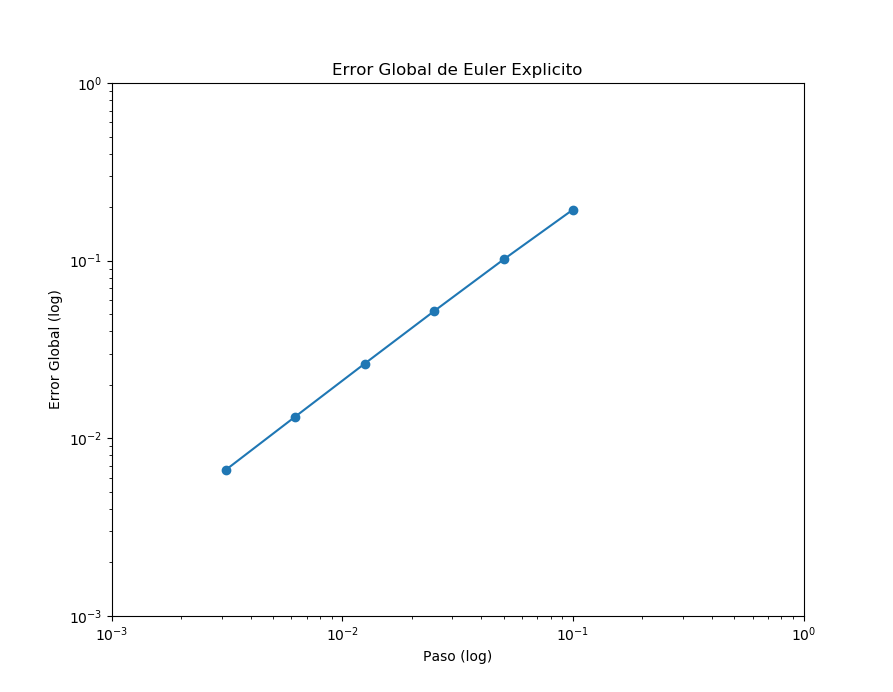
\includegraphics{fig 1.2.png}
    \end{center}
    
    Podemos observar que, en escala logaritmica, el error global y el paso
tienen una relacion lineal, que es lo esperado de un metodo con error
global de orden \(O(h)\).

\section*{Ejercicio 2}

Tomando el PVI (\ref{eq:1}) y la solución general de la ecuación
(\ref{eq:2}) del ejercicio anterior aplicaremos el método del Trapecio
explícito con paso \(h_1=0.1\). En el ejercicio 1 se argumentó la
existencia y unicidad del PVI.

Calculemos el error global en el punto t = 1:
\[E_{Trapecio}(h_1)=\left|w_{10}-y(1) \right|\] con \(w_{10}\) la
aproximación del método en t=1.

    \begin{Verbatim}[commandchars=\\\{\}]
{\color{incolor}In [{\color{incolor}1}]:} \PY{n}{f} \PY{o}{=} \PY{k}{lambda} \PY{n}{t}\PY{p}{,} \PY{n}{y} \PY{p}{:} \PY{n}{y}\PY{o}{+}\PY{l+m+mi}{2}\PY{o}{*}\PY{n}{np}\PY{o}{.}\PY{n}{exp}\PY{p}{(}\PY{o}{\PYZhy{}}\PY{n}{t}\PY{p}{)}
        \PY{n}{exact} \PY{o}{=} \PY{k}{lambda} \PY{n}{t}\PY{p}{,} \PY{n}{t0}\PY{p}{,} \PY{n}{y0} \PY{p}{:} \PY{n}{np}\PY{o}{.}\PY{n}{exp}\PY{p}{(}\PY{n}{t}\PY{p}{)}\PY{o}{*}\PY{p}{(}\PY{n}{y0}\PY{o}{*}\PY{n}{np}\PY{o}{.}\PY{n}{exp}\PY{p}{(}\PY{o}{\PYZhy{}}\PY{n}{t0}\PY{p}{)}\PY{o}{+}\PY{n}{np}\PY{o}{.}\PY{n}{exp}\PY{p}{(}\PY{o}{\PYZhy{}}\PY{l+m+mi}{2}\PY{o}{*}\PY{n}{t0}\PY{p}{)}\PY{o}{\PYZhy{}}\PY{n}{np}\PY{o}{.}\PY{n}{exp}\PY{p}{(}\PY{o}{\PYZhy{}}\PY{l+m+mi}{2}\PY{o}{*}\PY{n}{t}\PY{p}{)}\PY{p}{)}
        \PY{n}{I} \PY{o}{=} \PY{p}{(}\PY{l+m+mi}{0}\PY{p}{,} \PY{l+m+mi}{1}\PY{p}{)}
        \PY{n}{y0} \PY{o}{=} \PY{l+m+mi}{1}
        \PY{n}{y1} \PY{o}{=} \PY{n}{exact}\PY{p}{(}\PY{l+m+mi}{1}\PY{p}{,}\PY{l+m+mi}{0}\PY{p}{,}\PY{l+m+mi}{1}\PY{p}{)}
        \PY{n}{T}\PY{p}{,} \PY{n}{W} \PY{o}{=} \PY{n}{odesolver}\PY{o}{.}\PY{n}{solve}\PY{p}{(}\PY{n}{f}\PY{p}{,}\PY{n}{y0}\PY{p}{,}\PY{n}{I}\PY{p}{,}\PY{l+m+mi}{10}\PY{p}{,}\PY{n}{method}\PY{o}{=}\PY{l+s+s2}{\PYZdq{}}\PY{l+s+s2}{Explicit Trapezoid}\PY{l+s+s2}{\PYZdq{}}\PY{p}{)}
        \PY{n}{globalError} \PY{o}{=} \PY{n+nb}{abs}\PY{p}{(}\PY{n}{W}\PY{p}{[}\PY{l+m+mi}{0}\PY{p}{,}\PY{l+m+mi}{10}\PY{p}{]}\PY{o}{\PYZhy{}}\PY{n}{y1}\PY{p}{)}
\end{Verbatim}
   
    $$E_{Trapecio}(h_1)= 0.0046374955401011775$$
    
    Veamos lo que sucede cuando usamos el paso \(h_2:=\frac{h_1}{2}=0.05\) y
calculemos el correspondiende error global en t=1:
\[E_{Trapecio}(h_2)=\left|w_{20}-y(1) \right|\]

    \begin{Verbatim}[commandchars=\\\{\}]
{\color{incolor}In [{\color{incolor}2}]:} \PY{n}{T}\PY{p}{,} \PY{n}{W} \PY{o}{=} \PY{n}{odesolver}\PY{o}{.}\PY{n}{solve}\PY{p}{(}\PY{n}{f}\PY{p}{,}\PY{n}{y0}\PY{p}{,}\PY{n}{I}\PY{p}{,}\PY{l+m+mi}{20}\PY{p}{,}\PY{n}{method}\PY{o}{=}\PY{l+s+s2}{\PYZdq{}}\PY{l+s+s2}{Explicit Trapezoid}\PY{l+s+s2}{\PYZdq{}}\PY{p}{)}
        \PY{n}{globalError} \PY{o}{=} \PY{n+nb}{abs}\PY{p}{(}\PY{n}{W}\PY{p}{[}\PY{l+m+mi}{0}\PY{p}{,}\PY{l+m+mi}{20}\PY{p}{]}\PY{o}{\PYZhy{}}\PY{n}{y1}\PY{p}{)}
\end{Verbatim}
   
    $$E_{Trapecio}(h_2)= 0.0012209778161409446$$
    
    Ahora calcuemos el error global en t=1 usando el método Runge-Kutta 4
usando \(h_1=0.1\) : \[E_{RK4}(h_1)=\left|w_{10}-y(1) \right|\]

    \begin{Verbatim}[commandchars=\\\{\}]
{\color{incolor}In [{\color{incolor}3}]:} \PY{n}{T}\PY{p}{,} \PY{n}{W} \PY{o}{=} \PY{n}{odesolver}\PY{o}{.}\PY{n}{solve}\PY{p}{(}\PY{n}{f}\PY{p}{,}\PY{n}{y0}\PY{p}{,}\PY{n}{I}\PY{p}{,}\PY{l+m+mi}{10}\PY{p}{,}\PY{n}{method}\PY{o}{=}\PY{l+s+s2}{\PYZdq{}}\PY{l+s+s2}{RK4}\PY{l+s+s2}{\PYZdq{}}\PY{p}{)}
        \PY{n}{globalError} \PY{o}{=} \PY{n+nb}{abs}\PY{p}{(}\PY{n}{W}\PY{p}{[}\PY{l+m+mi}{0}\PY{p}{,}\PY{l+m+mi}{10}\PY{p}{]}\PY{o}{\PYZhy{}}\PY{n}{y1}\PY{p}{)}
\end{Verbatim}

    $$E_{RK4}(h_1)= 2.334812125859287e-06$$
    
    \begin{table}[h]
\centering
\begin{tabular}{|l|lll|}
\hline
                                   & E$_{Trapecio}(h_1)$   & E$_{Trapecio}(h_2)$   & E$_{RK4}(h_1)$                       \\ \hline
Error (global en t = 1)            & 4.63749554010 $\times$ 10$^{-3}$& 1.22097781614 $\times$ 10$^{-3}$& 2.3348121258 $\times$ 10$^{-6}$ \\
N\'umero de estados & 20                    & 40                    & 40                                  \\ \hline
\end{tabular}
\end{table}

    En la tabla anterior notamos lo siguiente:
\[E_{RK4}(h_1)<E_{Trapecio}(h_2)<E_{Trapecio}(h_1)\]

    Podemos observar que mediante el método del Trapecio explícito con paso
\(h_2\) obtenemos un error aproximadamente 4 veces menor que con paso
\(h_1\) ya que: \[E_{Trapecio}(h_1)=O(h_1^2)\]
\[   \Rightarrow E_{Trapecio}(h_2)=O(h_2^2)=O\left(\frac{h_1}{2}\right)^2\]
\[ \Rightarrow E_{Trapecio}(h_2) \approx \frac{1}{4}O(h_1^2)=\frac{1}{4}E_{Trapecio}(h_1) \]
El problema es que el método con \(h_2\) necesita de 40 estados, el
doble con respecto a usar \(h_1\).

    Por otro lado, el método Runge-Kutta 4 necesita de 40 estados al igual
que el Trapecio explícito con \(h_2\) pero observando los resultados de
la tabla notamos que el error global \(E_{RK4}\) es menor a
\(E_{Trapecio}(h_2)\) por un factor de \(10^3\) aproximadamente.

    Por lo tanto, para reducir el error, es preferible usar el método
Runge-Kutta 4 ya que, por los mismos 40 estados requeridos, se obtiene
un error menor al del Trapecio explícito con \(h_2\).

\section*{Ejercicio 3}

Tomemos el siguiente PVI:

\begin{equation} \label{eq:3}
 \begin{array}{c} y_1' = - y_1 + y_2 \\
y_2' =- y_1 - y_2 \end{array} 
\qquad \mbox{con} \qquad \begin{array}{c}
y_1(0)=0 \\ y_2(0)=1 \end{array} \qquad \mbox{para } t\in [0,1] \qquad 
\end{equation}
Con solución exacta
\(\overrightarrow{y}(t)=\left(\begin{array}{c} y_1(t) \\ y_2(t)\end{array} \right)\)
dada por :

\begin{equation} \label{eq:4}
 \begin{array}{c} y_1(t) = e^{-t}\sin(t) \\
y_2(t) = e^{-t}\cos(t) \end{array}
\end{equation}

    Sea \(\overrightarrow{W}_j\) el vector de aprximación correspondiente a
la aplicación del método del Punto Medio Implícito con paso \(h_j\). La
entrada \(w_i\) es la aproximación en \(t=1\) de \(y_i\) para
\(i,j \in \{1,2\}\). Definimos \(E_{PMImpl}(h_j)=\Vert G_j \Vert _2\) el error
global en \(t=1\) para \(j \in \{1,2\}\), con \(\overrightarrow{G}_j:=\vert W_j-\overrightarrow{y}(1) \vert\)
\(\quad\) cuya entrada \(g_i=\vert w_1-y_i(1) \vert\).

    Aplicaremos el método para \(h_1=0.1\) y \(h_2=0.01\):

    \begin{Verbatim}[commandchars=\\\{\}]
{\color{incolor}In [{\color{incolor}1}]:} \PY{n}{f} \PY{o}{=} \PY{k}{lambda} \PY{n}{t}\PY{p}{,} \PY{n}{y} \PY{p}{:} \PY{n}{np}\PY{o}{.}\PY{n}{array}\PY{p}{(}\PY{p}{[}\PY{o}{\PYZhy{}}\PY{n}{y}\PY{p}{[}\PY{l+m+mi}{0}\PY{p}{]}\PY{o}{+}\PY{n}{y}\PY{p}{[}\PY{l+m+mi}{1}\PY{p}{]}\PY{p}{,} \PY{o}{\PYZhy{}}\PY{n}{y}\PY{p}{[}\PY{l+m+mi}{0}\PY{p}{]}\PY{o}{\PYZhy{}}\PY{n}{y}\PY{p}{[}\PY{l+m+mi}{1}\PY{p}{]}\PY{p}{]}\PY{p}{)}
        \PY{n}{soln} \PY{o}{=} \PY{k}{lambda} \PY{n}{t}\PY{p}{:} \PY{n}{np}\PY{o}{.}\PY{n}{array}\PY{p}{(}\PY{p}{[}\PY{n}{np}\PY{o}{.}\PY{n}{exp}\PY{p}{(}\PY{o}{\PYZhy{}}\PY{n}{T}\PY{p}{)}\PY{o}{*}\PY{n}{np}\PY{o}{.}\PY{n}{sin}\PY{p}{(}\PY{n}{T}\PY{p}{)}\PY{p}{,} \PY{n}{np}\PY{o}{.}\PY{n}{exp}\PY{p}{(}\PY{o}{\PYZhy{}}\PY{n}{T}\PY{p}{)}\PY{o}{*}\PY{n}{np}\PY{o}{.}\PY{n}{cos}\PY{p}{(}\PY{n}{T}\PY{p}{)}\PY{p}{]}\PY{p}{)}
        \PY{n}{y0} \PY{o}{=} \PY{n}{np}\PY{o}{.}\PY{n}{array}\PY{p}{(}\PY{p}{[}\PY{l+m+mi}{0}\PY{p}{,}\PY{l+m+mi}{1}\PY{p}{]}\PY{p}{)}
        \PY{n}{T}\PY{p}{,}\PY{n}{W} \PY{o}{=} \PY{n}{odesolver}\PY{o}{.}\PY{n}{solve}\PY{p}{(}\PY{n}{f}\PY{p}{,} \PY{n}{y0}\PY{p}{,} \PY{p}{(}\PY{l+m+mi}{0}\PY{p}{,}\PY{l+m+mi}{1}\PY{p}{)}\PY{p}{,} \PY{l+m+mi}{10}\PY{p}{,} \PY{n}{method} \PY{o}{=} \PY{l+s+s1}{\PYZsq{}}\PY{l+s+s1}{Implicit Midpoint}\PY{l+s+s1}{\PYZsq{}}\PY{p}{)}
        \PY{n}{globalError1}\PY{o}{=}\PY{n}{linear}\PY{o}{.}\PY{n}{norm}\PY{p}{(}\PY{n}{W}\PY{p}{[}\PY{p}{:}\PY{p}{,}\PY{l+m+mi}{10}\PY{p}{]}\PY{o}{\PYZhy{}}\PY{n}{soln}\PY{p}{(}\PY{n}{T}\PY{p}{)}\PY{p}{[}\PY{p}{:}\PY{p}{,}\PY{l+m+mi}{10}\PY{p}{]}\PY{p}{)}
        \PY{n}{dif}\PY{o}{=}\PY{n+nb}{abs}\PY{p}{(}\PY{n}{W}\PY{p}{[}\PY{p}{:}\PY{p}{,}\PY{l+m+mi}{10}\PY{p}{]}\PY{o}{\PYZhy{}}\PY{n}{soln}\PY{p}{(}\PY{n}{T}\PY{p}{)}\PY{p}{[}\PY{p}{:}\PY{p}{,}\PY{l+m+mi}{10}\PY{p}{]}\PY{p}{)}
\end{Verbatim}
\begin{align*}
    h_1&=0.1 \\ 
 \vec{W_1}&= 
\begin{pmatrix} 
0.310408 \\ 
0.198583 \\ 
\end{pmatrix}\\
 \vec{G_1} &= 
\begin{pmatrix} 
0.000848 \\ 
0.000183 \\ 
\end{pmatrix}\\
 E_{PMImpl}(h_1) &= 0.0008678198131427709
\end{align*}
    

    \begin{Verbatim}[commandchars=\\\{\}]
{\color{incolor}In [{\color{incolor}2}]:} \PY{n}{T}\PY{p}{,}\PY{n}{W} \PY{o}{=} \PY{n}{odesolver}\PY{o}{.}\PY{n}{solve}\PY{p}{(}\PY{n}{f}\PY{p}{,} \PY{n}{y0}\PY{p}{,} \PY{p}{(}\PY{l+m+mi}{0}\PY{p}{,}\PY{l+m+mi}{1}\PY{p}{)}\PY{p}{,} \PY{l+m+mi}{100}\PY{p}{,} \PY{n}{method} \PY{o}{=} \PY{l+s+s1}{\PYZsq{}}\PY{l+s+s1}{Implicit Midpoint}\PY{l+s+s1}{\PYZsq{}}\PY{p}{)}
        \PY{n}{globalError2}\PY{o}{=}\PY{n}{linear}\PY{o}{.}\PY{n}{norm}\PY{p}{(}\PY{n}{W}\PY{p}{[}\PY{p}{:}\PY{p}{,}\PY{l+m+mi}{100}\PY{p}{]}\PY{o}{\PYZhy{}}\PY{n}{soln}\PY{p}{(}\PY{l+m+mi}{1}\PY{p}{)}\PY{p}{[}\PY{p}{:}\PY{p}{,}\PY{l+m+mi}{100}\PY{p}{]}\PY{p}{)}
        \PY{n}{dif}\PY{o}{=}\PY{n+nb}{abs}\PY{p}{(}\PY{n}{W}\PY{p}{[}\PY{p}{:}\PY{p}{,}\PY{l+m+mi}{100}\PY{p}{]}\PY{o}{\PYZhy{}}\PY{n}{soln}\PY{p}{(}\PY{n}{T}\PY{p}{)}\PY{p}{[}\PY{p}{:}\PY{p}{,}\PY{l+m+mi}{100}\PY{p}{]}\PY{p}{)}
\end{Verbatim}
\begin{align*}
    h_2&=0.01 \\ 
 \vec{W_2} &= 
\begin{pmatrix} 
0.309568 \\ 
0.198764 \\ 
\end{pmatrix}\\
 \vec{G_2} &= 
\begin{pmatrix} 
0.000008 \\ 
0.000002 \\ 
\end{pmatrix}\\
 E_{PMImpl}(h_2) &= 8.671073839286167e-06
\end{align*}
    

    Sabemos que el método del Punto Medio Implícito con paso $ \hat{h} $ tiene un
error global de de orden 2. Luego, con \(\hat{h}:=h_1=0.1\) esperamos:
\[E_{PMImpl}(h_1)=O\left ( h_1^2 \right ) = O \left( 0.1^2 \right)\]
Y con \(\hat{h}:=h_2=0.01\) esperamos:
\[E_{PMImpl}(h_2)=O\left ( h_2^2 \right ) = O \left( 0.01^2 \right)\]

    Observamos que: \[E_{PMImpl}(h_1)=O\left ( h_1^2 \right ) \]
\[  h_2= \frac{h_1}{10}   \Rightarrow      E_{PMImpl}(h_2) =O\left(\frac{h_1}{10}\right)^2 
\Rightarrow E_{PMImpl}(h_2) \approx \frac{1}{100}O(h_1^2)=\frac{1}{100}E_{PMImpl}(h_1) \]

    Esto implica que el error global del método para \(h_2\) debe ser
aproximadamente 100 veces menor al error global con el paso \(h_1\). Comparemos esto con nuestros resultados:

\[ E_{PMImpl}(h_2)=8.671073839286167e−06 \approx 8.67819813142771e−06= \frac{1}{100}E_{PMImpl}(h_1) \]

Y vemos que en efecto la reducción del error de \(h_1\) a \(h_2=\frac{h_1}{10}\) es consistente con la teoria.

\section*{Ejercicio 4}



\section*{Ejercicio 5}

Consideremos el PVI (\ref{eq:1}), cuya solucion (\ref{eq:2}) ha sido
justificada previamente. Utilizemos los métodos:

\begin{itemize}
    \item Euler Explícito
    \item Trapecio Explícito
    \item Punto Medio Explícito 
    \item RK4 
\end{itemize}
Con pasos \(h\in\{1/50,1/100,1/200\}\) para calcular y comparar el error
global en t=1. Obtenemos como resultados:

\begin{tabular}{{c|r r r r}} 
 \hline 
Paso & Euler Explicito & Trapecio Explicito & Punto Medio Implicito & Runge-Kutta 4 \\ \hline 
0.02 & 0.041788516341 & 0.000201525212813 & 0.00031786426130 & 4.138891895e-09 \\ 
0.01 & 0.0210985428547 & 5.090600531e-05 & 8.0138760276e-05 & 2.61991317529e-10 \\ 
0.005 & 0.010601086125 & 1.27925873654e-05 & 2.01192086386e-05 & 1.64810387559e-11 \\ 
\hline 
 \end{tabular}

    \begin{center}
    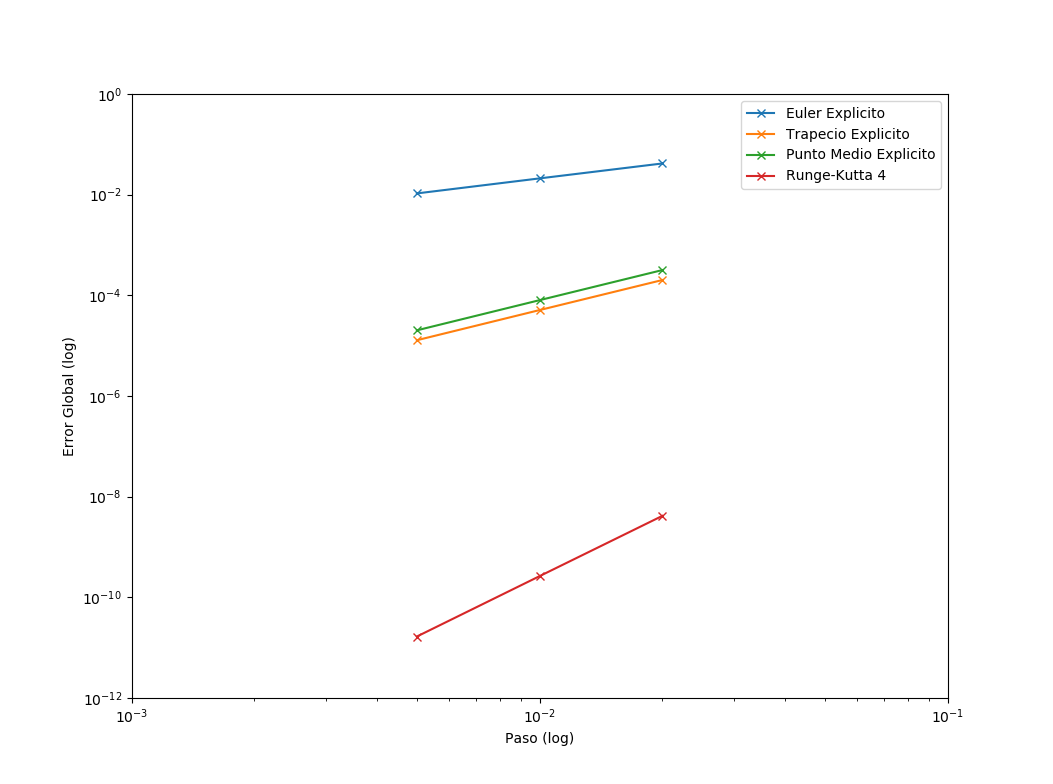
\includegraphics{fig 5.1.png}
    \end{center}
    
    En la tabla podemos notar los Errores Globales en t=1 de cada método
coinciden con los órdenes que vimos teóricamente (\(O(h)\) para Euler,
\(O(h^2)\) para Trapecio y Punto Medio y \(O(h^4)\) para RK4). También
podemos notar que a pesar de tener el mismo orden, el método del
trapecio fué más preciso que el método del punto medio para esta ODE.

La gráfica de nuevo confirma esto, pues vemos que la pendiente
aproxiamda de las rectas de los errores coinside con sus errores
teoricos.

\section*{Ejercicio 6}

Tomemos el siguiente PVI:

\begin{align*}y'' &= 10y' (1 - y)
\\ y(0)&=1 \\ y(1) &= 1 - \frac{\pi}{20}
\end{align*}

Para $t \in [0,1]$. Luego podemos reescribirlo como un sistema de ecuaciones de primer orden de la siguiente manera:

\begin{align*} y_1' &= y_2 \\
y_2' &= 10 y_2 (1 - y_1) 
\end{align*}

Con solución exacta dada por :

\begin{equation}
 \begin{array}{c} 
     y(t) = 1-\frac{\pi}{20} \tan(\frac{\pi}{4}t) \\
     y(1) = 1-\frac{\pi}{20}
 \end{array} 
\end{equation}

Así, definimos f como

    \begin{Verbatim}[commandchars=\\\{\}]
{\color{incolor}In [{\color{incolor}1}]:} \PY{n}{f} \PY{o}{=} \PY{k}{lambda} \PY{n}{t}\PY{p}{,} \PY{n}{y} \PY{p}{:} \PY{n}{np}\PY{o}{.}\PY{n}{array}\PY{p}{(}\PY{p}{[}\PY{n}{y}\PY{p}{[}\PY{l+m+mi}{1}\PY{p}{]}\PY{p}{,} \PY{l+m+mi}{10}\PY{o}{*}\PY{n}{y}\PY{p}{[}\PY{l+m+mi}{1}\PY{p}{]}\PY{o}{*}\PY{p}{(}\PY{l+m+mi}{1}\PY{o}{\PYZhy{}}\PY{n}{y}\PY{p}{[}\PY{l+m+mi}{0}\PY{p}{]}\PY{p}{)}\PY{p}{]}\PY{p}{)}
        \PY{n}{exact} \PY{o}{=} \PY{k}{lambda} \PY{n}{t} \PY{p}{:} \PY{l+m+mi}{1}\PY{o}{\PYZhy{}}\PY{n}{pi}\PY{o}{/}\PY{l+m+mi}{20}\PY{o}{*}\PY{n}{tan}\PY{p}{(}\PY{n}{pi}\PY{o}{/}\PY{l+m+mi}{4}\PY{o}{*}\PY{n}{t}\PY{p}{)}
\end{Verbatim}


    Para aplicar Shooting Method, tomamos una aproximación inicial de
\(y_2 = 1\)

\[\overrightarrow{y_0}(t) = \left(\begin{array}{c} y_1(t) \\
y_2(t)\end{array} \right) = \left( \begin{array}{c} 1
\\ 0 \end{array} \right)\]

y utilizaremos el método de Runge Kutta 4 con 1000 pasos para aproximar
la función en \(y(1)\)

    \begin{Verbatim}[commandchars=\\\{\}]
{\color{incolor}In [{\color{incolor}2}]:} \PY{n}{y0} \PY{o}{=} \PY{p}{[}\PY{l+m+mi}{1}\PY{p}{,} \PY{l+m+mi}{0}\PY{p}{]}
        \PY{n}{\PYZus{}}\PY{p}{,} \PY{n}{W} \PY{o}{=} \PY{n}{odesolver}\PY{o}{.}\PY{n}{solve}\PY{p}{(}\PY{n}{f}\PY{p}{,} \PY{n}{y0}\PY{p}{,} \PY{p}{(}\PY{l+m+mi}{0}\PY{p}{,}\PY{l+m+mi}{1}\PY{p}{)}\PY{p}{,} \PY{l+m+mi}{1000}\PY{p}{,}  \PY{n}{method} \PY{o}{=} \PY{l+s+s1}{\PYZsq{}}\PY{l+s+s1}{rk4}\PY{l+s+s1}{\PYZsq{}}\PY{p}{)}
        \PY{n}{ans} \PY{o}{=} \PY{n}{W}\PY{p}{[}\PY{l+m+mi}{0}\PY{p}{]}\PY{p}{[}\PY{o}{\PYZhy{}}\PY{l+m+mi}{1}\PY{p}{]}
\end{Verbatim}
$$W_{1000} = 1.0$$
Veamos que tan acertada fue nuestra elección
$$ W_{1000} - y(1)  = 0.15707963267948966$$

Parece ser que nuestra aproximación inicial sobreestimó la solución.
Usaremos el método de Newton para seguir generando aproximaciones.

Definimos una función \(F : \mathbb{R} \rightarrow \mathbb{R}\) que toma
una estimación inical de \(y_2 = y'\) y regresa la distancia a la
solución delimitada por el BVP. De este modo, $F(0) = 0.15707963267948966$
    En \emph{odesolver}, definimos la función "shooting" que toma una
función, un valor inicial de \(y_1\), una aproximación inicial de
\(y_2\) y la la solución del BVP y crea la función F, para después
aplicar el método de Newton hasta encontrar una raíz, o bien, encontrar
el valor inicial de \(y_2\) que hace que se satisfaga el BVP. Esto nos da la siguiente tabla:

\begin{center}
\begin{tabular}{c| r r}
\hline
Iteracion & Pendiente & Error \\
\hline
1 & -0.1571058117415369 & 0.06011796937074976 \\
2 & -0.1136129484483078 & 0.015605062058363206 \\
3 & -0.12257599202933653 & 0.0012971130776441298 \\
4 & -0.1233885530092585 &  3.0275526610390457e-05 \\
5 & -0.1233700198445987 & 5.7558321331363516e-08 \\
6 & -0.12337005501206845 & 2.5480728638171968e-12 \\
\hline
\end{tabular}
\end{center}

Observamos que con esta aproximación inicial se satisface el BVP con un error menor a 1e-10. Ademas, podemos observar el comportamiento del error y las pendientes aproximadas en las siguientes graficas:

    \begin{center}
    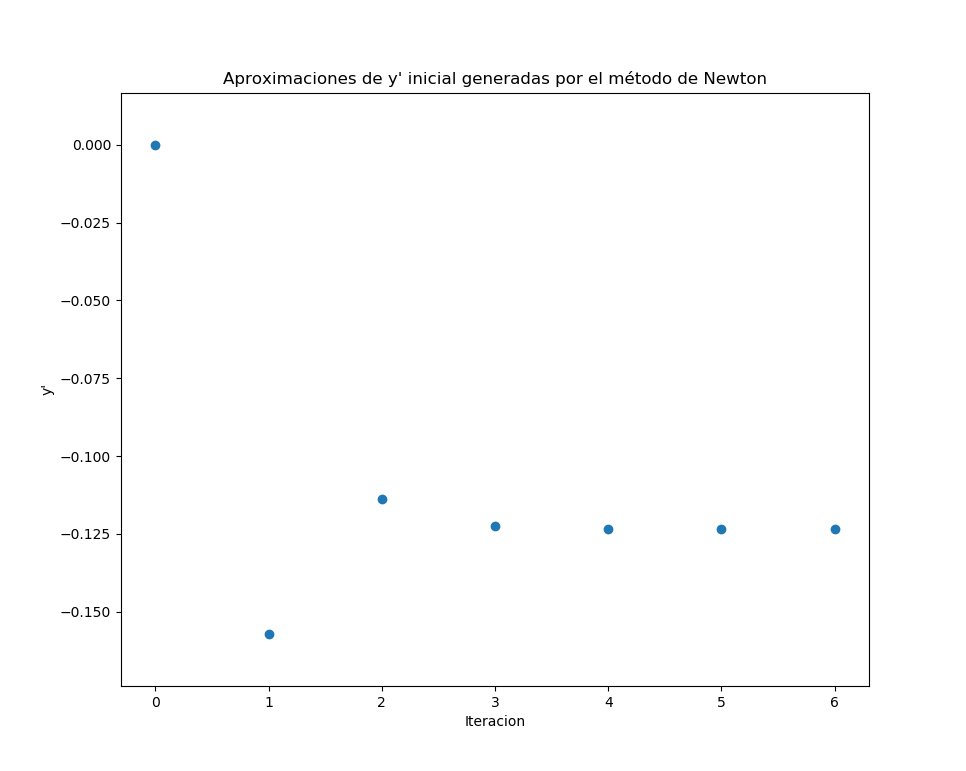
\includegraphics{fig 6.1.png}
    \end{center}
    
   \begin{center}
    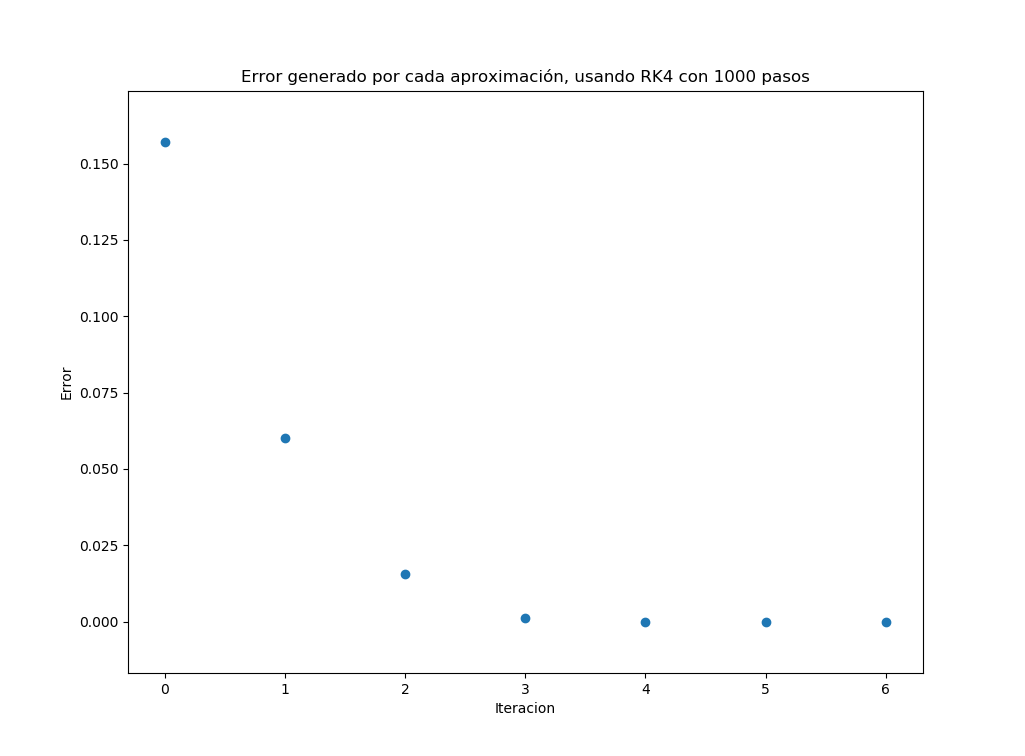
\includegraphics{fig 6.2.png}
    \end{center}

    % Add a bibliography block to the postdoc
    
    
    
    \end{document}
